\title{PLUTO simulation and imaging procedures}
\author{Jonathan Rogers}
\date{\today}
\documentclass[12pt]{article}

\usepackage{graphicx}
\usepackage{amsmath}
\usepackage{verbatim}
\usepackage{subcaption}

\usepackage{listings}
\usepackage{color}

\definecolor{dkgreen}{rgb}{0,0.6,0}
\definecolor{gray}{rgb}{0.5,0.5,0.5}
\definecolor{mauve}{rgb}{0.58,0,0.82}

\lstset{frame=tb,
	language=Python,
	aboveskip=3mm,
	belowskip=3mm,
	showstringspaces=false,
	columns=flexible,
	basicstyle={\small\ttfamily},
	numbers=none,
	numberstyle=\tiny\color{gray},
	keywordstyle=\color{blue},
	commentstyle=\color{dkgreen},
	stringstyle=\color{mauve},
	breaklines=true,
	breakatwhitespace=true,
	tabsize=3
}

\begin{document}
\maketitle

\noindent This document outlines the general processes required to simulate a 2D astrophysical jet using PLUTO. It also provides general instructions on imaging this simulation using python. \\
\newline
Note that it is assumed that the user has python 2.7 installed. Python 3 is not compatible pyPLUTO, a python module that comes with PLUTO.
\section{PLUTO}

PLUTO is a user-friendly finite-volume/area, shock-capturing code that was written (in C) to integrate a set of conservation laws such as the hydrodynamical equations. There are four inbuilt physics modules allowing for hydrodynamical, magnetohydrodynamical, special relativistic hydrodynamical, and relativistic magnetohydrodynamical physics to be investigated.\\
\\
After the initial installation (which is beyond the scope of this document), the code requires 4 files to run: init.c, definitions.h, pluto.ini and an appropriate makefile for your OS. The following sections summarise the role of these files, and give a brief how-to on setting up your own simulation with an emphasis on producing astrophysical jets. The latter sections discuss imaging your simulation using python. A more in-depth guide to PLTUO can be found in the userguide at http://plutocode.ph.unito.it/files/userguide.pdf.

Euler equations:\\
conservation of mass:
conservation of momentum
conservation of energy
In conservative form:
\begin{equation}
\frac{\partial}{\partial t} \begin{pmatrix}
\rho \\
m_{1} \\
m_{2} \\
m_{3} \\
E \\
\end{pmatrix}
 = -\nabla\cdot
 \begin{pmatrix}
 \rho\vec{u}\\
 m_{1}\vec{u} + P\vec{E_1}\\
 m_{2}\vec{u} + P\vec{E_2}\\
 m_{3}\vec{u} + P\vec{E_3}\\
 (E + P)\vec{u}
 \end{pmatrix}
 -
 \begin{pmatrix}
 0\\
 \rho \frac{\partial}{\partial x_{1}}\Phi\\
 \rho \frac{\partial}{\partial x_{2}}\Phi\\
 \rho \frac{\partial}{\partial x_{3}}\Phi\\
 \rho \vec{u} \cdot \nabla\Phi
 \end{pmatrix}
\end{equation}
m is the momentum density (rho $\vec{u}\vec{u}$).
Which is of the form
\begin{equation}
\frac{\partial}{\partial t}\vec{U} = -\nabla \cdot T(\vec{U}) - S(\vec{U})
\end{equation}
is this a rieman problem?
\subsection{Simulation set up}

The three important files that govern the behaviour of your simulation are the definitions.h, pluto.ini and init.c files. These files define things such as:
\begin{itemize}
	\item Complexity of the physics
	\item resolution
	\item input parameter values
	\item Grid print timestep size
	\item simulation run time
	\item user defined boundary conditions
\end{itemize}
 The files are not independent of each other - that is, there are options that are 'switched on' in one file, but given a value in another. The details of important parameters in these files are discussed below. Note that not all parameters and flags are discussed, only those needed to set up a simple HD, 2D jet simulation.

\subsubsection{definitions.h}
The definitions.h file specifies:
\begin{itemize}
	\item which fluid equations will be solved
	\item what Rieman solver and time stepping technique to use
	\item any user defined parameters
\end{itemize}
any other physics dependent parameters (most of which won't be discussed) such as:
\begin{itemize}
	\item the equation of state
	\item inclusion of entropy in conservation laws
\end{itemize}
 
The definitions.h file can be configured by running the setup.py script (located in the PLUTO/ folder by default). However, there are some parameters (namely those which are physics dependent) that must be edited manually.

\paragraph{Physics and geometry}\mbox{}
\newline
Most parameters at the beginning of the definitions.h file are somewhat self-explanatory. 
\begin{itemize}
\item DIMENSIONS  determines the number of dimensions in your simulation. For 2D simulations, trivially the DIMENSIONS parameters takes the integer value 2. 

\item COMPONENTS is the total number of vector components of the simulation. For example, if ignoring magnetic fields, a 2D simulation may only have a velocity field (which is only a function of (x,y)), and therefore COMPONENTS should be set to 2. Generally COMPONENTS = DIMENSIONS.

\item GEOMETRY specifies the geometry of your simulation and requires a string. Each spatial coordinate is labelled as x$_1$, x$_2$, and x$_3$ respectively, and can take one of four values:
\subitem - Cartesian
\subitem - Cylindrical
\subitem - Polar
\subitem - Spherical
The importance of selecting the most appropriate geometry is discussed further in section 2.

\item PHYSICS is used to select which physics module you want to use. The available modules are given in section 1. Setting this parameter to HD invokes classical hydrodynamics as described by the Euler equations (see section 6.1 of the user guide for more information).

\item BODY\_FORCE is a switch that enables for a body force term to be included in the momentum and energy equations. It can be input as a scalar potential, or expressed as a vector. This will be discussed further in 'the init.c section'. This is an important flag as it invokes self-gravity of the gas in the simulation which can drastically change the resulting morphology.
\end{itemize}

\paragraph{Solvers}
The solvers block 

\begin{itemize}
\item RECONSTRUCTION
The code works by solving the equations of fluid dynamics in vectorized form. This is done so using Godunov's theorem (getreference). This particular method is chosen as it has proved important "wikipedia: in the  development of high resolution schemes for the numerical solutions to partial differential equations.". 
The method also guarantees a solution to the entropy equation (if convergence).

For more on Godunov's method, see **get a reference, maybe wikipedias one?**

During the use of Godunov's method, for time step n, the cell average of the solution vector to your system of conservation equations is calculated. The manner in which this cell average is calculated can determine how physically realistic your simulation is.

Figure x shows the cell average solution to U (red dot) as is solved over your spatial grid. The red lines illustrate how the solution curve is reconstructed between the cells. The blue dot is the interpolated value given the different type of reconstruction schemes.

\subitem - Figure (x a) shows a flat reconstruction. Quite clearly there are discontinuities in the solution curve. This is realistic for primitive variables that may have discontinuities present. For example, astrophysical jets may show a bow shock present, characterised by a near discontinuous change in in the pressure, density, and temperate. It is the least computative expensive reconstructor.

\subitem - Figure (x b) shows a linear reconstruction. This will still model a discontinuity well, whilst better approximating continuous parts of the function.

\subitem - Figure (x c) shows a parabolic interpolation. 
This smooths the solution curve, which should not be expected to involve a discontinuity. Parabolic interpolation gives a higher spatial accuracy of the solution over the grid. However, due to the smooth nature of the interpolation, extreme variation in values is not interpolated well.

\begin{figure}[h]
	\centering
	\begin{subfigure}[b]{0.45\textwidth}
		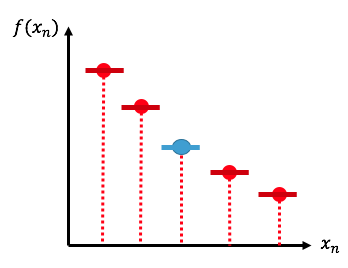
\includegraphics[width=\textwidth]{flat_recon}
		\caption{change the planes of the images to Ux vs (x1,x2) plane. change blue line to red in this one too.}
	\end{subfigure}
	\begin{subfigure}[b]{0.45\textwidth}
	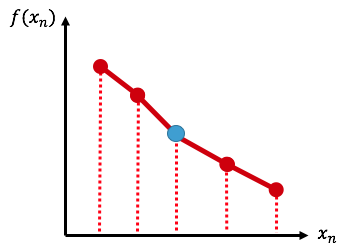
\includegraphics[width=\textwidth]{linear_recon}
	\caption{change the planes of the images to Ux vs (x1,x2) plane}
	\end{subfigure}
	\begin{subfigure}[b]{0.45\textwidth}
	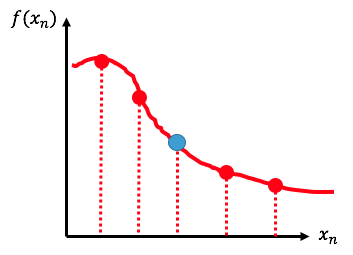
\includegraphics[width=\textwidth]{parabolic_recon}
	\caption{change the planes of the images to Ux vs (x1,x2) plane}
	\end{subfigure}		
\end{figure}

The advantage of the high resolution shock capturing method that PLUTO uses is that linear or parabolic reconstruction is used everywhere - except where discontunities are present. Discontinuous parts of the solution are instead reconstructed using a flat scheme. This ensures solutions are of higher spatial resolution where available This is set by the limiter flag. 

\item TIME\_STEPPING
The timestepping scheme used in solving the Euler equations can be set with the TIME\_STEPPING parameter. The userguide outlines the pros and cons of the different combinations of recontructors and time steppers, which change depending on the geometry of your simulation. For the remainder of this document, we are going to assume a second-order Runge-Kutter timestepper, or RK2, with linear reconstruction.
\end{itemize}

\paragraph{Defining parameters}
\begin{itemize}
\item NTRACER essentially adds a colour to the fluid particles. The zero-th tracer (tr0)  is one that is continuously injected. Further tracer particles can be added to inject at customisable times, each being given a consecutive value in its variable name. This is useful to determine where the bulk electron population resides as a function of injection time (i.e. how is disperses), which when weighted by the pressure, is proportional to the intensity? (check this..). 

\subitem - The maximum number of tracers accepted when running setup.py is 8, any more and you will need to manually edit the definitions.h file after running setup.py. The inbuilt GUI is not optimized for more than 8 instances of tracer injections. Attempting to image such a simulation with the GUI will result in not being able to see the colour map of your solution vector.

\item USER\_DEF\_PARAMETERS is the number of parameters that have been defined in the pluto.ini and init.c file. For more info on this parameter see sub/section x.x and x.x 

\item The pysics dependent declarations will, for simplicity, assume that the gas behaves as an ideal gas. This is done by setting the equation of state (EOS) to IDEAL.

\item The user defined paramaters block is where each new variable that is required in the simulation is defined. The number of variables here must match the value of USER\_DEF\_PARAMETERS, as well as the number defined in the pluto.ini file.

 \item PRINT\_TO\_FILE , when given the value YES, outputs the log of the simulation to a file named pluto.log. This file is extremely useful for troubleshooting and should always be switched on.
\end{itemize}

\subsubsection{pluto.ini}

On execution of the code, pluto checks for an input file named pluto.ini. This file contains the run-time information for the simulation. The information includes the spatial domain of the grid, temporal parameters such as the simulation length and output frequency, and values for any user defined parameters.

The pluto.ini file is also where Adaptive mesh refinement (AMR) and output parameters associated with this are configured. AMR is a tool that changes the size of your grid where finer resolution is required. AMR is not discussed here.

\paragraph{Grid}\mbox{}
\newline
 The [Grid] section enables for resolution customisation over the simulation grid space. Finer cell spacings may be required in some areas of jet simulations. For example:
 
 \begin{itemize}
  \item A larger resolution is often required close to the injection point of your jet, otherwise the jet may not accurately (or at all) propagate onto the grid.
  
  
 \item In areas around the jet-environment boundary, a higher resolution grid is needed to be able to resolve turbulence. This is vitally important as turbulence plays a large role in momentum transfer from jets, causing differing morphologies (e.g. Perucho DATE). 
 \end{itemize}
The simulation grid is composed of 'grid patches'. Each grid patch may differ in:- 
\begin{itemize}
\item Size
\item Number of cells
\item Size of the cells comprising the patch; or
\item How the cells are distributed over the patch
\end{itemize}For example, Figure 2  shows a 2D grid space extending out to x = 8.  There are 2 patches (as indicated by the shading). Patch 1 is defied over 0 $\leq x < 4$ and 0 $\leq y < 4$  (resolution of 4x4).

Patch 2 has half the resolution of patch one, and covers the domain 4 $\leq x <$ 8, and 4 $\leq y <$ 8. 
This is useful if finer resolution is only needed on smaller scales. The computation time benefits from the smaller grid only being defined in part of the simulation.

\begin{figure}[h]
	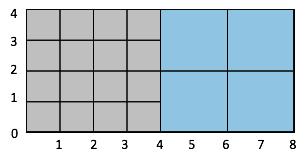
\includegraphics[width=8cm]{gridspaces}
	\centering
	\caption{A mock grid with two patches, highlighted in brown and blue.}
\end{figure}

\paragraph{Time and Solver blocks}\mbox{}
\newline
- Includes comes values that relate to the time stepper selected in the definitions.h file. See the userguide for more info.

- tstop is the integration stop time (i.e. simulation temporal length)

- first\_dt sets the initial time step. Values that are too extreme may cause stability issues at the very beginning on the integration. As per the useguide, a typical value is 10$^{-6}$

see table 4.1 for appropriate solvers for your chosen physics module.
\paragraph{Boundary}\mbox{}
\newline

need to figure out a way to not just copy the userguide for this bit 

- mention that a reflective boundary mimics the existence of a counter jet, thus giving a more accurate simulation.

\paragraph{Static grid output}\mbox{}
\newline
- Controls the output frequency and the format. 
- Only going to worry about the dbl line.
- dbl, print step, whats -1?, single\_file or multiple\_files, depending on if you want all of your variables printed to the one file?

\paragraph{Parameters}\mbox{}
The parameters section is where values are given to the user defined parameters. Values of these parameters are used in the init.c file.
\newline


\subsubsection{init.c}
The initial conditions and boundary conditions of the problem are set in the init.c file. Here we briefly discuss the functions involved. The manipulation of the lower (x,y) boundary (or lower (r) boundary on a spherical grid) to include an inflow of conserved simulation quantities is used to simulate a fluid jet. Quantities involved may also be user defined parameters (values set in the pluto.ini file)

User defined parameters are assigned to variables by var = g\_inputParam[PAR], where PAR is the same of the parameter as set in the definitions.h and pluto.ini files.\\
\\
The syntax used to define a state variable is d->Vc[PRS][k][j][i], where pressure = PRS. The velocity in each coordinate can be set be replacing PRS with VX1, VX2, or VX3. The initial density is set using the variable RHO.

\paragraph{Init section}
The init "section"? (not sure what to call it) defines the initial condition of the state variables in each cell over the grid. These conditions are therefore functions of coordinates (which will vary depending on the coordinate system).\\
\\
This "section"? may involve defining variables such as $c_s$, and the adiabatic index, $\gamma$. An example of this section is used in Section 2.\\

\paragraph{UserDefBoundary section}
The UserDefBoundary function is switched on if, in the pluto.ini file, a boundary value is set to USER\_DEF\_BOUNDARY.

It is also useful to define a pressure floor (code shit beds if negative pressures are involved) in boundary conditions. can do this using the function TOP\_LOOP.
\begin{lstlisting}[language=C++]
if (side == 0){
	TOT_LOOP(k,j,i){
		if (d->Vc[PRS][k][j][i] < 1.e-6) /* set min pressure */
		{
		d->Vc[PRS][k][j][i] = 1.e-6;
		}
	}
}
\end{lstlisting}
Top loop loops over every cell in the simulation.\\
\\
What does d$->$ Vc actually do? What is side==0? may need to ask ross.\\
d->Vc[PRS][k][j][i] is the syntax needed to define a state variable value.

BOX\_LOOP
"The macro BOX LOOP(box,k,j,i) performs a loop over the bottom boundary zones and, for cellcentered
data, it is equivalent to the macro X2 BEG LOOP(k,j,i)"
Loops over the boundary values only.
An example of using the BOX LOOP function to set a boundary condition is shown in Section 2.

\subsection{Nondimensionalization of the simulation}
Two limitations of numerical simulations are computation time, and numerical integration error. Both of these factors can minimised by writing optimised code that uses less memory.\\
\\
Arithimic using large numbers is both computationaly expensive and uses more memory. This issue can be addressed by normalising simulation parameters in the init.c file, named the state variables $\rho$, P and $v_{jet}$. The ratio of the length normalisation unit to the sound speed in the environment gives the physical time step of your simulation. This is therefore the unit time, corresponding to 1 in the code units (tstop in the pluto.ini? file therefore being the age of your jet). Furthermore, normalising the length scale to characteristic scales can also be useful. Typical scales are discussed below.

An example of nondimensionalization is given in section 2 (using jupyter notebook with Python 2.7).

\subsubsection{Characteristic length scales of astrophysical jets}

Krause et al. 2012 outlines the method and arguments leading to these length scales.

There are two bounding length scales to consider referred to as L1 and L2. L1 is the distance from the AGN that the jet density approaches the environment density, i.e.
\begin{equation}
\text{L1: }\rho_{jet} = \rho_x
\end{equation}
This is typically referred to as the inner scale. This can be expressed in terms of the jet power, Q$_0$, jet velocity, v$_{jet}$ and $\rho_{jet}$ (Alenxader 2006). 

\begin{equation}
L1 = 2\sqrt{2}\left(\frac{Q_0}{\rho_x v_{jet}^3} \right)^{1/2}
\end{equation}

The outer scale of a jet, or L2 is where the jet pressure is comparable to the environment pressure, i.e.
\begin{equation}
\text{L2: }P_{jet} = P_{x}
\end{equation}
Note that the environment pressure and density could refer to the ambient medium, or the jet cocoon should one have formed. This can be expressed in terms of $Q_0$, $\rho_x$, and the soundspeed of the medium $c_x$ (Komissarov \& Falle 1998)
\begin{equation}
GIVE EQUATION
\end{equation}
\\
There exist three more length scales between L1 and L2. However, unlike the inner and outer scale, the order of the remaining three scales depend on the physics of the jet and environment, and will determine the morphological features of the jet and the surrounding medium. These three intermediate scales relate to the locations of jet collimation (L1a), cocoon formation (L1b) and jet termination (L1c). The order to these three scales change with jet morphology, and thus jet morphology can be understood via the ratios of the scales. These scales discussed should be taken as order of magnitude estimates rather than exact physical locations in simulations or observations.

\paragraph{L1a: Scale of jet collimation}
Collimation happens on scales where the sideways ram pressure of the jet starts to fall below the environmental pressure. I.e.
\begin{equation}
\rho_{jet}v_{jet}^{2}\sin{\theta} < P_{x}
\end{equation}
Where subscript \textit{x} refers to the environment immediately outside the jet, and $\theta$ is the half opening angle of the jet.\\
\\
\paragraph{L1b: Scale of cocoon formation}
The scale on which the jet density falls below the density of the environment. Should a cocoon form before the jet collimates (i.e. L1a/L1b < 1), then for the purposes of L1a, the subscript x refers to the cocoon.\\
\\
\paragraph{L1c: Scale of jet termination}
A jet termination shock appears on scales of L1c. At L1c, the forward ram pressure of the jet falls below the environmental density. Should the scale of L1b be smaller than L1c, then this environment refers to the cocoon.\\
\\
Krause et al. 2012 discusses the derivation of these length scales in some detail, calling on work from Komissarov \& Falle 1998, and Alexander 2006. However, the length scales calculated relate to an environment of constant density. Hardcastle \& Krause 2013 used these length scales in numerical modelling of radio galaxy globes in cluster (non-constant) environments. This however, is beyond the goals of this tutorial.

\subsection{Viewing your data}
There is an pre-coded GUI that uses the pyPLUTO python module to display 2D images, or slices of your simulation output. However, the resolution at which the GUI displays the data is less than the actual resolution of the simulation (this is usually the case when the grid spacing is low enough to resolve turbulence). It is easier to get a better quality image by importing the pyPLUTO module into pluto yourself, and manually extracting, then imaging the data yourself. This section outlines how to use the pyPLUTO code, how to create images, and a small introduction to making movies of your simulations.

\subsubsection{pyPLUTO module}
pyPLUTO is a pluto module developed by Bhargav Vaidya and Denis Stepanovs, and is extremely useful for analysing PLUTO simulations. Within the module is the function pload, which creates a pyPLUTO object with attributes that include the output matrices of your simulation, grid information and information on the simulated quantities. The function requires two inputs:
\begin{itemize}
\item ns: the output file number (eg, 0 would be the output binary file data.0000.dbl)
\item run\_dir: the directory that your simulation resides in
\end{itemize}
For example, to load the density map of your simulation:
\begin{lstlisting}
import pyPLUTO as pp

ns = 1 #define output file to analyse
run_dir = 'MyDirectory/MyPlutoSimulation/' #set run directory
curObject = pp.pload(ns,run_dir) #create pyPLUTO object
density = curObject.rho #get attribute (density in this case) from the pyPLUTO object
X1_AXIS = curObject.x1 #get x axis of simulation, is a vector
X2_AXIS = curObject.x2 #get y axis of simulation, is a vector
\end{lstlisting}
It is often useful to define simulations of astrophysical jets in spherical coordinates (see section x), in which case the X1\_vector and X2\_vector would actually represent the (R,$\Theta$) axes.\\
is there ay more to say?

\subsubsection{Plotting with matplotlib}

Set up a grid using meshgrid
\begin{lstlisting}
import numpy as np
import matplotlib.pyplot as plt

#Create a grid by producing a 2D array of the combination of the values in the two *_AXIS vectors
X1, X2 = np.meshgrid(X1_AXIS, X2_AXIS)

#Create the density map using the pcolormesh plotting function 
plt.pcolormesh(X1,X2,density)

#Set axis lavels
plt.xlabel('x [code units]')
plt.ylabel('y [code units]')

#Add a colorbar
cb = plt.colorbar()

#Display the plot
plt.show()
\end{lstlisting}

Alternatively, is it better practise to write functions for getting the data and plotting it. An example of this is given in section 2.

\section{PLUTO Example (github required)}

The following section works through setting up and imaging a simple 2D HD simulation of an astrophysical jet using the PLUTO code, and jpython 2.7

We begin by obtaining the necessary run files using github.



Require the user to download some example files from gitgub
- probably also talk about how to put your own files on github, giving special care not to prompt the user to upload their entire simulation.



An example of an FR-II jet will be produced using a density profile that declines as a function of $r^{2}$. The simulation must therefore be defined in spherical coordinates. This is consistent with the definitions.h and pluto.ini file.

The grid block in the pluto.ini file reflects a quarter quarter of a circle. We will set a variable resolution in r, and an even resolution in theta.

- Define new parameters (make a diagram)
- go through the init.c file and code up each section
- run the code
- image the code using the code in the section before
- plot in R,Theta space, then transform to cartesian and replot
- should look like this: pic goes here
- congrats, you've got a jet.


- the geometry and body force selection must match the coding of your simulation in the init.c file
- can specify opening angle of jet in terms of theta (mention Krause et al. 2012 and how it is a morpholoy divide between jets)

-have pretty much written this example - just need to copy my python code.

\subsection{}
TO DO ON MY AUSCOPE SHIFT :D (hopefully..)
- copy jet example
- download the init.c, definitions.h and pluto.ini file from github
- define  H\_OPEN\_ANG
- define  MACH\_EXT


\end{document}